\section{Lagrangefunktionen}
Generelt er Newtons love gode i deres simplicitet, med let forståelse af dem og deres anvendelse. Det er relativt simpelt at forestille sig en kraft, der skubber noget i en bestemt retning. En af ulemperne ved dem er dog, at man er afhænging af begrænsningskræfter, så som snorkræfter, normalkræfter og lignende, der er svære at definere og håndtere, for at beskrive den fysiske virkelighed. Det er dog mulig at slippe af med disse kræfter, ved at benytte en anden formalisme til at beskrive klassisk mekanik. Dette svarer så at sige til at skifte værktøjskasse: de redskaber man benytter er anderledes, men det færdige resultat bliver det samme.
%problemløsningen ofte er en slavisk proces, der kræver at man tager højde for alle kraftpåvirkninger på ens system, og kan gøre systemet mere kompliceret end det er. Et eksempel på dette er systemer, hvis bevægelse har restriktioner fra snorkræfter, normalkræfter eller lignende, der ikke udfører arbejde på systemet. Her menes der, at netop disse ``constrained forces'' sætter begrænsninger på, hvordan systemet kan bevæge sig, men at de i sig selv ikke tilføjer eller fratager energi fra systemet. Newtons love kræver dog, at de inkluderes i udregningerne for at kunne beskrive systemet korrekt. \\

% Her introduceres fordelen ved 
Den formalisme vi vil arbejde med hedder Lagrangeformalismen, og den tager udgangspunkt i en undersøgelse af et systems kinetiske og potentielle energi. Ud fra disse kan man opskrive differentialligninger, der, ligesom for Newtonsk mekanik (Newtons 2. lov), beskriver systemet. I Lagrangeformalismen arbejder man aldrig med kræfter, hvilket på den ene side betyder, at man slipper af med de problematiske begrænsningskræfter. Det betyder så også, at i den formulering, der introduceres her, ikke kan beskrive gnidningskræfter, luftmodstand og lignende. En yderligere fordel ved Lagrangeformalismen af klassisk mekanik er at den kan genereliseres til at beskrive alt fysik lige fra generel relativitetsteori til kvantemekanik og kvantefeltteori.
%, hvordan man opsætter differentialligninger for systemet, da $\sum\va{F} = m\va{a} = m\ddot{\va{r}}$). Ulempen ved Lagrangemekanik, i formen der introduceres her er, at den kun gælder for systemer udelukkende påvirket af konservative kræfter. Dette inkluderer derved ikke gnidningskræfter, luftmodstand og lignende.

Systemet undersøges ud fra en funktion kaldet Lagrangefunktionen, der betegnes med symbolet $L$, og defineres som
%
\begin{align} \label{mek:eq:Lagrange_funktion}
	L = K - V.
\end{align}
%
I \cref{mek:eq:Lagrange_funktion} er $K$ systemets kinetiske energi, og $V$ er systemets potentielle energi.

\subsection*{Euler-Lagrangeligningen i kartesiske koordinater}
Først vil vi beskrive vores energier ud fra kartesiske koordinater, som derefter kan konverteres over til mere favorable, generaliserede koordinater, som vælges specifikt for hvert system. Disse gør normalt problemet lettere at løse. %Vi vil desuden tage udgangspunkt i et system uden bundne kræfter (snorkraft, normalkraft), hvor vi senere kan gøre det mere generelt. \\
Den kinetiske energi for en punktpartikel er
%
\begin{align}\label{mek:eq:Kinetisk_kartesisk}
	K = \frac{1}{2} m v^2 = \frac{1}{2} m \left(\dot{\va{r}}\right)^2 = \frac{1}{2} m (\dot{x}^2 + \dot{y}^2 + \dot{z}^2),
\end{align}
%
og den potentielle energi er specifikt for systemet, men afhænger af de tre kartesiske koordinater:
%
\begin{align}\label{mek:eq:Potentiel_kartesisk}
	V = V(\va{r}) = V(x,y,z).
\end{align}
%
Med Lagrangefunktionen opskrevet skal vi nu bruge en måde at frembringe bevægelsernes differentialligninger for systemet. Dette gøres ud fra Euler-Lagrangeligningerne:
%
\begin{equation} \label{mek:eq:el_kartesisk}
\begin{aligned}
	\dv{}{t} \left( \pdv{L}{\dot{x}} \right) &= \pdv{L}{x}, \\%[0.75em]
	\dv{}{t} \left( \pdv{L}{\dot{y}} \right) &= \pdv{L}{y}, \\%[0.75em]
	\dv{}{t} \left( \pdv{L}{\dot{z}} \right) &= \pdv{L}{z}.
\end{aligned}
\end{equation}
%
Der fremgår altså en ligning til at udregne systemets bevægelsesligning for hver af de tre kartesiske koordinater, ud fra differentiation af Lagrangefunktionen. Ligesom Newtons anden lov, \cref{mek:eq:N2}, blev betragtet som en byggesten, hvorpå resten af mekanikken hviler, så kan Euler-Lagrangeligningerne, \cref{mek:eq:el_kartesisk}, også ses som en byggesten Lagrangeformalismen hviler på. Det er værd at holde tungen lige i munden, når man skal udregne disse. Blandt andet skal det noteres, at der indgår to forskellige partielle differentiationer af $L$, samt en totaldifferentiation med hensyn til tiden. Når der står $\pdv*{L}{x}$ menes der her, at man skal partielt differentiere $L$ med hensyn til $x$. Det betyder, at man skal betragte $x$ som værende den eneste variabel $L$ afhænger af, og se alle andre led som konstanter (det vil sige at eventuelle tidsafledte led $\dot{x}$ også skal ses som konstante, da der ikke eksplicit står $x$). Ydermere skal man ignorere, at $x$ også kan afhænge af tiden. Hvad så når der står $\pdv*{L}{\dot{x}}$? Her skal man i stedet betragte $\dot{x}$ som værende det eneste varierende led, og differentiere med hensyn til det. Derfor skal alle andre led, $x$, $y$, $\dot{y}$ og så videre ses som konstanter, når der differentieres. Slutteligt, så skal der totaldifferentieres med hensyn til tiden. Her skal den nye funktion $\pdv*{L}{\dot{x}}$ differentieres på traditionel vis med hensyn til tiden. Men det er ikke garanteret, at der eksplicit står et $t$-led nogle steder. Det skal dog huskes, at vores funktion har mulighed for at afhænge af $x,y,z,\dot{x},\dot{y},\dot{z}$, som hver især kan afhænge af tiden $t$. Derfor kan totaldifferentiationen gennemføres ved at betragte leddene $x,y,z,\dot{x},\dot{y},\dot{z}$ som funktioner, der også skal differentieres med hensyn til tiden. Det kan være en god idé at genopfriske disse pointer fra \cref{mat:ex:part_diff,mat:ex:part_tot_diff} i \cref{chap:matematik}.
%Kunne godt bruge et kort eksempel før vi går videre til generaliserede koordinater
%

En interessant bemærkning er faktisk, at det relativt let kan vises at Newtons 2. lov og Euler-Lagrangeligningerne er ækvivalente.%(hvilket forhåbentligt også skulle være tilfældet, da det er ækvivalente løsningsmetoder, som begge kan bruges til at komme frem til de relevante bevægelsesligninger for et system).
Betragt eksempelvis $x$-koordinatet. Her fås to funktioner ved at partielt differentiere med hensyn til hhv. $x$ og $\dot{x}$:
%
\begin{align}
	\pdv{L}{x} &= \pdv{}{x} \Big( K(\dot{x},\dot{y},\dot{z}) - V(x,y,z) \Big), \\%[0.75em]
	\pdv{L}{\dot{x}} &= \pdv{}{\dot{x}} \Big( K(\dot{x},\dot{y},\dot{z}) - V(x,y,z) \Big).
\end{align}
%
Her har vi, at kun $V$ afhænger eksplicit af $x$, mens $K$ kun eksplicit afhænger af $\dot{x}$. Derved fås de to resultater:
%
\begin{align}
	\pdv{L}{x} &= - \pdv{V}{x} = F_x, \label{mek:eq:newton_kraft_lagrange}\\%[0.75em]
	\pdv{L}{\dot{x}} &= \pdv{K}{\dot{x}} = \pdv{}{\dot{x}}\left(\frac{1}{2} m \left(\dot{x}^2+\dot{y}^2+\dot{z}^2\right)\right) = m\dot{x} \label{mek:eq:newton_impuls_lagrange}% = p_x, 
\end{align}
%
I Newtonsk mekanik er potential energi defineret således at den totale kraft i $x$-retningen er $F_x = -\partial V/\partial x$, hvilket er brugt i \cref{mek:eq:newton_kraft_lagrange}. Differentiere \cref{mek:eq:newton_impuls_lagrange} total med hensyn til tiden fås
%
\begin{align}
    \dv{}{t} \left( \pdv{L}{\dot{z}} \right) &= \dv{}{t} m\dot{x} = m\ddot{x}. \label{mek:eq:newton_acceleration_lagrange}
    %
    \intertext{Kombineres \cref{mek:eq:el_kartesisk,mek:eq:newton_kraft_lagrange,mek:eq:newton_impuls_lagrange} fås $x$-komposanten af Newtons anden lov}
    %
    F_x &= m\ddot{x}.
\end{align}

%Koordinaterne anvendt vil således være generaliserede koordinater $q_i$ $(q_1,q_2,...,q_n)$, som hver i sær udelukkende afhænger af tiden.
\subsection*{Euler-Lagrangeligningen i generaliserede koordinater}
Med den nyfundne forståelse for Lagrangefunktionen og Euler-Lagrangeligningen i kartesiske koordinater vil vi nu undersøge tilfældet, hvor vi i stedet anvender generaliserede koordinater. Fra afsnittet om generaliserede koordinater har vi, at generaliserede koordinater $(q_1,q_2,...,q_n)$ er et valgt koordinatsæt, hvor antallet af koordinater svarer til antallet af frihedsgrader for systemet. Det vil sige, at hvis vi kan nøjes med at beskrive systemet med et enkelt koordinat, som i tilfældet med det simple pendul, så har vi et generaliseret koordinat (som i dette eksempel ville være oplagt at vælge som pendulvinklen $\phi$). 
% Her vil vi så have $n$ Euler-Lagrangeligninger, hvor $n$ er antallet af frihedsgrader for systemet, og derved antallet af generaliserede koordinater. På baggrund af \cref{mek:eq:newton_kraft_lagrange} kaldes $\pdv*{L}{q_i}$ for den i'te komponent af den generaliserede kraft. Da \cref{mek:eq:newton_impuls_lagrange} kan skrives som
% %
% \begin{align}
%     \pdv{L}{\dot{x}} = m\dot{x} = p_x,
% \end{align}
% %
% hvor $p_x$ er $x$-komposanten af impulsen, kaldes $\pdv*{L}{\dot{q}_i}$ for den i'te komponent af den generaliserede impuls. Disse er ikke garanteret at være den fysiske kraft og impuls, som vi forstår dem, men er nærmere hvad vi ækvivalent kan forstå som dem i vores generaliserede koordinater (hvilket er grunden til navnet).
I genereliserede koordinater er Euler-Lagrangeligningerne
%
\begin{align} \label{mek:eq:Euler-Lagrange}
	\dv{}{t} \left( \pdv{L}{\dot{q_i}} \right) = \pdv{L}{q_i}, \quad i = \{1,2,...,n\}.
\end{align}
%
% eller i ord:
% %
% \begin{align}
% 	\text{(generaliseret kraft)} = \text{(ændringsrate i generaliseret impuls)}.
% \end{align}
Euler-Lagrangeligningerne ser ud på samme måde i kartesiske og generaliserede koordinater, men der er dog forskelle. I det kartesiske tilfælde vil alle led, der har noget med hastigheder og accelerationer være på venstre side af \cref{mek:eq:el_kartesisk}, mens alt hvad der har noget med stedkoordinater at gøre, vil være på højre side. Specielt vil de to typer aldrig blandes -- led som $x\dot{x}$ dukker ikke op. Kort sagt står alt med prikker til venstre, alt uden prikker til højre og man blander aldrig noget uden prikker med noget, der har en eller flere prikker. I generaliserede koordinater er dette ikke sandt, og så snart man har med krumme koordinatsystemer at gøre, så ser man hyppigt at den kinetiske energi også afhænger af stedkoordinatet. Det så vi eksempelvis med polære koordinater, hvor hastigheden afhænger af radiuskoordinatet (se \cref{mek:eq:SmartFart}).

\begin{figure}[]
	\centering
	\begin{tikzpicture}[line width=2pt]
        \coordinate (m) at (2.25,-5);
        \coordinate (o) at (0,0);
        %
    	\fill [pattern = north east lines] (-3.5,0) rectangle (3.5,0.5);
        %
        \draw (-3.5,0) to (3.5,0);
        \draw (o) to (m);
    	\draw (1.2,-2.5) node[anchor=west]{\LARGE $l$};
        %
        \fill (m) circle (3.5pt);
        \draw (o) node[anchor=center]{\huge $\boldsymbol{\times}$};
        %
        \draw[-{Stealth[length=4mm, width=2.5mm]}] (-3,-0.75) to (-1.75,-0.75);
    	\draw[-{Stealth[length=4mm, width=2.5mm]}] (-3,-0.75) to (-3,-2);
    	\draw (-2.4,-1.4) node[anchor=center]{\Large $\bigotimes$};
    	%
    	\draw (-2.5,-0.75) node[anchor=south]{\LARGE $\vu{x}$};
    	\draw (-3,-1.5) node[anchor=east]{\LARGE $\vu{y}$};
    	\draw (-2.25,-1.35) node[anchor=west]{\LARGE $\vu{z}$};
    	%
        \draw[dashed, line width=1pt] (o) to (0,-6.5);
        \draw[dashed, line width=1pt] (0,-5) to (m);
    	\draw (1.125,-5) node[anchor=south]{\LARGE $x$};
    	\draw (0,-2.5) node[anchor=east]{\LARGE $y$};
    	%
    	\draw [domain=-90:-65.77, line width=1.5pt] plot ({cos(\x)}, {sin(\x)});
    	\draw (0.23,-1.25) node[anchor=center]{\LARGE $\phi$};
    	%
    	\draw[-{Stealth[length=4mm, width=2.5mm]}] (m) -- ++(24.23:1.25cm);
    	\draw[-{Stealth[length=4mm, width=2.5mm]}] (m) -- ++(-65.77:1.25cm);
     	\draw (2.2,-5.5) node[anchor=center]{\LARGE $\vu{r}$};
     	\draw (3.1,-5.05) node[anchor=center]{\LARGE $\vu*{\phi}$};
     	%
     	\draw[-{Stealth[length=3mm, width=2mm]}, line width=1.5pt]
     	    (2.9,-3.85) node[anchor = west]{\LARGE $m$} [bend right=25] to (2.275,-4.85);
     	%
     	\draw[-{Stealth[length=3mm, width=2mm]}, line width=1.5pt]
     	    (-0.9,-0.65) node[anchor = east]{\LARGE $\mathcal{O}$} [bend right=25] to (-0.1,-0.2);
        %
    	\draw [domain=-90:-65.77, line width=1pt, dashed] plot
    	    ({5.48*cos(\x)}, {5.48*sin(\x)});
    	\draw[{Stealth[length=2mm, width=1.5mm]}-{Stealth[length=2mm, width=1.5mm]},
    	    line width=1.5pt] (-0.15,-5) to (-0.15,-5.48);
     	\draw (-0.15,-5.2) node[anchor=east]{\LARGE $h$};
    \end{tikzpicture}
  %
% 	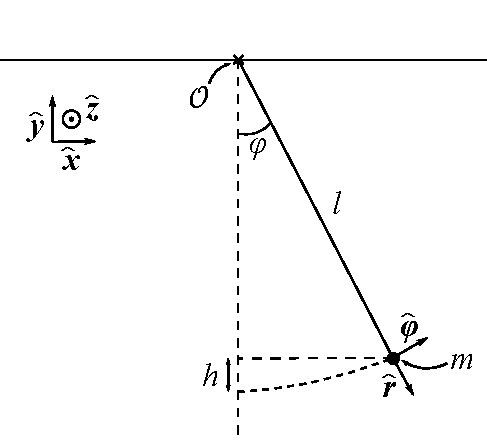
\includegraphics[width=.5\textwidth]{figurer/PendulLagrange.pdf}
	\caption{Samme pendul som i \cref{mek:fig:Pendul}. Pendulets højde, $h$, defineres ud fra nulpunktet for den potentielle energi, der vælges til at være pendulets ligevægtspunkt $(0,-l)$ (i kartesiske koordinater).}
	\label{mek:fig:PendulLagrange}
\end{figure}
%
\section{Eksempler på brugen af Lagrangemekanikken}
\begin{example}[Beskrivelse af pendul med Lagrangemekanik] \label{mek:ex:PendulLagrange}% Denne kommentar skal åbenbart være her for at undgå en grim indentering. Man kan også fjerne den med \noindent, men det er jo ligeså grimt
Igen kigges der på pendulet fra \cref{mek:ex:pendul_newton}, men denne gang gøres der brug af Lagrangemekanikken:
Først kigger vi på pendulet, hvis længde kaldes $l$, og massen af loddet for enden af snoren kaldes $m$. Der defineres et nulpunkt for pendulet, hvor lodet befinder sig, når pendulet er i hvile, altså når det hænger lodret ned, se \cref{mek:fig:PendulLagrange}.
Siden der kun er tale om en rotationel bevægelse, vælges et polært koordinatsystem. Den kinetiske energi af pendulet er givet ved
%
\begin{align}
	K &= \frac{1}{2} m v^2,
	%
    \intertext{hvor $v$ er lodets hastighed.
%for en rotationel bevægelse er givet ved pendulets længde $l$ og dets vinkelhastighed $\dot{\phi}$, 
    Fra \cref{mek:eq:SmartFart} vides det, at hastigheden afhænger af pendulets længde, $l$, og dets vinkelhastighed, $\dot{\phi}$. Den kinetiske energi bliver derved}
    %
	K &= \frac{1}{2} m (l \dot{\phi})^2. \label{mek:eq:pendul_k}
	%
    \intertext{Den potentielle energi er givet ved}
    %
	V &= mgh, \label{mek:eq:pendul_pot}
\end{align}
%
hvor $h$ er pendullodets højde over nulpunktet. Da nulpunktet er valgt som lodets placering i pendulets lodrette position kan denne højde skives som differensen af snorens længde og den korteste afstand imellem lodet og snoren. Bruges \cref{mat:eq:trig} kan man ved hjælp af den retvinklede trekant i \cref{mek:fig:PendulLagrange} vise at
%
\begin{align} \label{mek:eq:pendul_hoejde}
	h &= l - y = l - l \cos(\phi) = l \big( 1-\cos(\phi) \big).
\end{align}
%
Den potentielle energi bliver således ved kombination af \cref{mek:eq:pendul_pot,mek:eq:pendul_hoejde}
%
\begin{align} \label{mek:eq:pendul_v}
	V &= mgl \big( 1-\cos(\phi) \big).
\end{align}
%
I Lagrangefunktionen, \cref{mek:eq:Lagrange_funktion}, indsættes den kinetiske og den potentielle energi fra henholdsvis \cref{mek:eq:pendul_k} og \cref{mek:eq:pendul_v}, hvilket giver følgende:
%
\begin{align}
	L &= K - V = \frac{1}{2} m l^2 \dot{\phi}^2 - mgl(1-\cos(\phi)).
\end{align}
%
For at bruge Euler-Lagrangeligningen skal Lagrangefunktionen  differentieres nogle gange -- både totalt og partielt. Det kan hertil være nyttigt at kigge på \cref{mat:ex:part_tot_diff} i \cref{chap:matematik}. De partielt afledede af Lagrangefunktionen med hensyn til $\phi$ og $\dot{\phi}$ bliver
%
\begin{align}
	\pdv{L}{\phi} &= - mgl \sin(\phi), \label{mek:eq:pendul_pdv_phi} \\%[.5em]
	\pdv{L}{\dot{\phi}} &= m l^2 \dot{\phi}
	%
    \intertext{og findes den tidsafledte af den sidste ligning fås}
    %
    \dv{}{t} \left( \pdv{L}{\dot{\phi}} \right) &= m l^2 \ddot{\phi}. \label{mek:eq:pendul_dt}
    %
    \intertext{Indsættes \cref{mek:eq:pendul_pdv_phi,mek:eq:pendul_dt} i Euler-Lagrangeligningen, \cref{mek:eq:Euler-Lagrange}, fås følgende:}
    %
     \dv{}{t}\left(\pdv{L}{\dot{\phi}}\right) &= \pdv{L}{\phi} \nonumber \\
	\implies m l^2 \ddot{\phi} &= - mgl \sin(\phi).
	%
    \intertext{I ovenstående ligning isoleres vinkelaccelerationen $\ddot{\phi}$:}
    %
    \ddot{\phi} &= - \frac{g}{l} \sin(\phi).
    %
    \intertext{Antages det at pendulets udsving vil være små, da kan der gøres brug af Taylorudviklingen for $\sin(\phi)$ fra \cref{mat:tab:Taylorseries_table}, hvorved der fås}
    %
    \ddot{\phi} &\simeq - \frac{g}{l} \phi, \label{mek:eq:pendul_eom_lagrange}
\end{align}
%
hvilket er pendulligningen, \cref{mek:eq:PendulLigning}. Taylorudviklingen af sinus blev diskuteret i den Newtonske beskrivelse af pendulet, se \cref{mek:ex:pendul_newton}. Hvorfor skulle Lagrangeformalismen give en simplere måde at beskrive pendulet end den Newtons formalisme? Det svære ved Lagrangeformalismen er at få valgt nogle gode koordinater, samt at få differentieret rigtigt hele vejen igennem. Valget af koordinater er ikke anderledes i Newtonsk mekanik, men som fysiker differentierer man funktioner så ofte, at det lidt svarer til at køre på cykel -- når først man har lært, det behøver man ikke tænke ret meget over det\footnote{Faktisk differentierer man funktioner så ofte som fysiker, at nogle fysikere vil insistere på, at det er lettere end at regne med tal.}. Det at håndtere begrænsningskræfterne er til gengæld mindre systematisk, og det kan hurtigt blive meget svært at gøre rigtigt, hvis man har med et kompliceret system at gøre.
%Så snart man bliver god til at differentiere rigtig, og opskrive Euler-Lagrangeligningen i nogle gode koordinater, så er denne metode markant lettere at benytte - det er bare et spørgsmål om træning.
\end{example}

\begin{figure}[]
	\centering
	\begin{tikzpicture}[line width=2pt, scale=0.9]
        \coordinate (m) at (2.25,-5);
        \coordinate (o) at (0,0);
        %
        \draw (-3.75,0) to (3.75,0) to (3.75,-6.75) to (-3.75,-6.75) to (-3.75,0);
        \draw[-{Stealth[length=4mm, width=2.5mm]}] (o) to (0,1.5);
    	\draw (0,0.75) node[anchor=west]{\LARGE $\va{a}$};
        \draw (o) to (m);
    	\draw (1.2,-2.5) node[anchor=west]{\LARGE $l$};
    	%
        \draw[line width=1.25pt] (0, -6.9) to ++(0, -1);
    	\foreach \i in {1,...,10}
        {
        \draw[line width=1.25pt] (3.75/10 * \i, -6.9) to ++(0, {-1/2*(-\i/10 + 2)});
        \draw[line width=1.25pt] (-3.75/10 * \i, -6.9) to ++(0, {-1/2*(-\i/10 + 2)});
        }
        %
        \fill (m) circle (3.5pt);
        \draw (o) node[anchor=center]{\Huge $\boldsymbol{\times}$};
        %
        \draw[-{Stealth[length=4mm, width=2.5mm]}] (-3,-0.75) to (-1.75,-0.75);
    	\draw[-{Stealth[length=4mm, width=2.5mm]}] (-3,-0.75) to (-3,-2);
    	\draw (-2.4,-1.4) node[anchor=center]{\Large $\bigotimes$};
    	%
    	\draw (-2.5,-0.75) node[anchor=south]{\LARGE $\vu{x}$};
    	\draw (-3,-1.5) node[anchor=east]{\LARGE $\vu{y}$};
    	\draw (-2.25,-1.35) node[anchor=west]{\LARGE $\vu{z}$};
    	%
        \draw[dashed, line width=1pt] (o) to (0,-6.5);
        \draw[dashed, line width=1pt] (0,-5) to (m);
    	\draw (1.125,-5) node[anchor=south]{\LARGE $x$};
    	\draw (0,-2.5) node[anchor=east]{\LARGE $y$};
    	%
    	\draw [domain=-90:-65.77, line width=1.5pt] plot ({cos(\x)}, {sin(\x)});
    	\draw (0.23,-1.25) node[anchor=center]{\LARGE $\phi$};
    	%
    	\draw[-{Stealth[length=4mm, width=2.5mm]}] (m) -- ++(24.23:1.25cm);
    	\draw[-{Stealth[length=4mm, width=2.5mm]}] (m) -- ++(-65.77:1.25cm);
     	\draw (2.2,-5.5) node[anchor=center]{\LARGE $\vu{r}$};
     	\draw (3.1,-5.05) node[anchor=center]{\LARGE $\vu*{\phi}$};
     	%
     	\draw[-{Stealth[length=3mm, width=2mm]}, line width=1.5pt]
     	    (2.9,-3.85) node[anchor = west]{\LARGE $m$} [bend right=25] to (2.275,-4.85);
     	%
     	\draw[-{Stealth[length=3mm, width=2mm]}, line width=1.5pt]
     	    (-0.9,-0.65) node[anchor = east]{\LARGE $\mathcal{O}$} [bend right=25] to (-0.1,-0.2);
        %
    	\draw [domain=-90:-65.77, line width=1pt, dashed] plot
    	    ({5.48*cos(\x)}, {5.48*sin(\x)});
    	\draw[{Stealth[length=2mm, width=1.5mm]}-{Stealth[length=2mm, width=1.5mm]},
    	    line width=1.5pt] (-0.15,-5) to (-0.15,-5.48);
     	\draw (-0.15,-5.2) node[anchor=east]{\LARGE $h$};
    \end{tikzpicture}
    %
% 	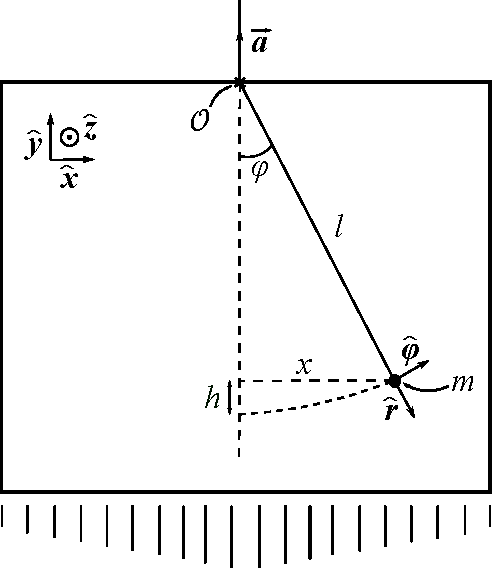
\includegraphics[scale=0.7]{figurer/PendulElevator.pdf}
	\caption{Samme pendul som i \cref{mek:fig:PendulLagrange}, dog nu placeret i en lineært accelererende elevator.}
	\label{mek:fig:PendulElevator}
\end{figure}
%
\begin{example}[Pendul med rotationel og translatorisk bevægelse] \label{mek:sec:elevator}% Denne kommentar skal åbenbart være her for at undgå en grim indentering. Man kan også fjerne den med \noindent, men det er jo ligeså grimt
Et anden godt eksempel på brugen af Lagrangeformalismen er situationen med et pendul i en elevator, hvilket er illustreret i \cref{mek:fig:PendulElevator}. Her bevæger lodet i pendulet sig ved en rotationel bevægelse, hvorimens elevatoren bevæger sig med en translatorisk bevægelse, hvilket her er ved konstant acceleration. At bevægelsen er translatorisk betyder at hele systemet deltager i bevægelsen. Det er ikke kun elevatoren -- pendulet følger med. Først skal stedfunktionen for elevatorens translatoriske bevægelse bestemmes. Der er her tale om bevægelse med konstant acceleration, hvilket kendes fra \cref{mat:ex:frit_fald} om frit fald i \cref{chap:matematik}. \Cref{mat:eq:position} giver at elevatorens $y$-koordinat, $y_\textup{el}$, er beskrevet af funktionen
%
\begin{align} \label{mek:eq:pendul_elevator_y_init}
	y_\textup{el}(t) &= \frac{1}{2}at^2 + v_{0,\textup{el}} t + y_{0,\textup{el}}.
\end{align}
%
Vælges lige præcis det koordinatsystem hvor $v_{0,\textup{el}} = y_{0,\textup{el}} = 0$ bliver \cref{mek:eq:pendul_elevator_y_init} til
%
\begin{align}
	y_\textup{el}(t) &= \frac{1}{2}at^2. \label{mek:eq:pendul_elevator_y}
	%
    \intertext{Herefter findes de kartesiske koordinaterne, $x$ og $y$, for loddet, udtrykt ved pendulets udsvingsvinkel, der bruges som generaliseret koordinat:}
    % samt de tidsafledede af disse:
    %
	x &= l \sin(\phi), \label{mek:eq:pendul_x} \\
	y &= l \big(1-\cos(\phi) \big) + \frac{1}{2} at^2, \label{mek:eq:pendul_i_elevator_y}
	%
	\intertext{\Cref{mek:eq:pendul_x} kommer fra den retvinklede trekant i \cref{mek:fig:PendulElevator}, mens \cref{mek:eq:pendul_i_elevator_y} fremkommer ved at lægge pendulets $y$-koordinat, \cref{mek:eq:pendul_hoejde}, sammen med elevatorens, \cref{mek:eq:pendul_elevator_y}. Differentieres \cref{mek:eq:pendul_x} med hensyn til tid fås}
	%
	\dot{x} &= l \cos(\phi) \dot{\phi}, \label{mek:eq:pendul_x_punkt} \\
	%
	\intertext{og tilsvarende fås for \cref{mek:eq:pendul_i_elevator_y}}
	%
	\dot{y} &= l \sin(\phi) \dot{\phi} + at. \label{mek:eq:pendul_y_punkt}
\end{align}
%
Systemets potentielle energi findes nu ved brug af \cref{mek:eq:pendul_x,mek:eq:pendul_i_elevator_y} til at være
%
\begin{align}
	V &= mgy = mg \left[ l \big( 1 - \cos(\phi) \big) + \frac{1}{2}at^2 \right],
\end{align}
%
mens \cref{mek:eq:pendul_x_punkt,mek:eq:pendul_y_punkt} giver at den kinetiske energi er
%
\begin{align}
&\begin{aligned}
	K &= \frac{1}{2} m \left( \dot{x}^2 + \dot{y}^2 \right) \\
	&= \frac{1}{2} m \left[ \Big( l^2 \cos^2(\phi) \dot{\phi} \Big) + \Big( l^2 \sin^2(\phi) \dot{\phi} + a^2t^2 + 2 l \sin(\phi) \dot{\phi} a t \Big) \right] \\
	&= \frac{1}{2} m \Big( l^2\phi^2 + a^2t^2 + 2l\sin(\phi)\dot{\phi}at \Big).
\end{aligned}
    %
    \intertext{Lagrangefunktionen bliver således}
    %
	L = K-&V = \frac{1}{2} m \Big( l^2\dot{\phi}^2 + a^2t^2 + 2l\sin(\phi)\dot{\phi}at \Big) - mg \left[ l \big( 1 - \cos(\phi) \big) + \frac{1}{2}at^2 \right].
\end{align}
%
De partielt afledede af Lagrangefunktionen i forhold til henholdsvis $\phi$ og $\dot{\phi}$, samt den tidsafledede af sidste findes:
%
\begin{align}
	\pdv{L}{\phi} &= ml\cos(\phi)\dot{\phi}at - mgl\sin(\phi), \\
	\pdv{L}{\dot{\phi}} &= ml^2\dot{\phi} + ml\sin(\phi)at, \\
	\dv{}{t}\left(\pdv{L}{\dot{\phi}}\right) &= ml^2\ddot{\phi} + ml\cos(\phi)\dot{\phi}at + ml\sin(\phi)a.
\end{align}
%
Indsættes dette i Euler-Lagrangeligningen fås
%
\begin{align} \label{mek:eq:pendul_elevator_eom1}
\begin{aligned}
	\pdv{L}{\phi} &= \dv{}{t}\left( \pdv{L}{\dot{\phi}} \right) \\
	 \implies ml\cos(\phi)\dot{\phi}at - mgl\sin(\phi) &= ml^2\ddot{\phi} + ml\cos(\phi)\dot{\phi}at + ml\sin(\phi)a.
\end{aligned}
\end{align}
%
Isoleres vinkelaccelerationen i \cref{mek:eq:pendul_elevator_eom1} fås
%
\begin{align}
	\ddot{\phi} &= - \frac{g+a}{l}\sin(\phi).
	%
    \intertext{Antages pendulets udsving at være lille, kan dette Taylorudvikles, ligesom i \cref{mek:ex:pendul_newton,mek:ex:PendulLagrange}, til}
    %
    \ddot{\phi} &\simeq - \frac{g+a}{l}\phi. \label{mek:eq:pendul_elevator_eom}
\end{align}
%
\Cref{mek:eq:pendul_elevator_eom} er på samme form som pendulligningen, \cref{mek:eq:pendul_eom,mek:eq:pendul_eom_lagrange}, hvorfor pendulet i elevatoren opfører sig som et almindeligt pendul, men hvor tyngdeacceleration er ændret til $\tilde{g} = g + a$. I dette tilfælde opfører elevatorens acceleration og tyndekraften sig på samme måde i forhold til pendulet, hvilket peger mod noget større -- nærmere bestemt ækvivalensprincippet fra generel relativitetsteori, hvilket der kan læses mere om i \cref{rel:sec:gr}.
\end{example}